\documentclass[12pt,a4paper]{article}
\usepackage[utf8]{vietnam}
\usepackage{amsmath,amssymb}
\usepackage{geometry}
\geometry{top=1.25cm,bottom=1.2cm,left=1.3cm,right=1.3cm,headheight=15pt,headsep=12pt,footskip=18pt}
\usepackage{tikz}
\usepackage{xcolor}
\usepackage{enumerate}
\usepackage{chemfig}
\usepackage[version=4]{mhchem}
\usepackage{fancyhdr}
\usepackage{ex_test}

\makeatletter
\@ifundefined{c@bt}{\newcounter{bt}}{}
\makeatother

\renewcommand{\baselinestretch}{0.91}
\setlength{\parskip}{0pt}

\definecolor{hfRed}{RGB}{211,47,47}
\definecolor{hfGreen}{RGB}{139,195,144}

% Header & Footer chuẩn theo ảnh Thầy cung cấp
\pagestyle{fancy}
\fancyhf{}
\fancyhead[L]{\small\itshape\color{hfRed} Tài liệu lưu hành nội bộ}
\fancyhead[R]{\small\itshape\color{hfRed} Thầy \textbf{TRẦN VĂN THẠNH} - 0777.470.803}
\renewcommand{\headrulewidth}{0.8pt}
\renewcommand{\headrule}{\hbox to\headwidth{\color{hfGreen}\leaders\hrule height \headrulewidth\hfill}}

\fancyfoot[L]{\small\itshape\color{hfRed} CS1: 6/15 Nguyễn Hoàng, P. Kim Long, TP Huế \quad|\quad CS2: 24 Đặng Thái Thân, TP Huế}
\fancyfoot[R]{\small\bfseries\color{hfRed} Trang \thepage}
\renewcommand{\footrulewidth}{0.8pt}
\renewcommand{\footrule}{\hbox to\headwidth{\color{hfGreen}\leaders\hrule height \footrulewidth\hfill}}

\fancypagestyle{firstpage}{
  \fancyhf{}
  \renewcommand{\headrulewidth}{0pt}
  \fancyfoot[L]{\small\itshape\color{hfRed} CS1: 6/15 Nguyễn Hoàng, P. Kim Long, TP Huế \quad|\quad CS2: 24 Đặng Thái Thân, TP Huế}
  \fancyfoot[R]{\small\bfseries\color{hfRed} Trang \thepage}
  \renewcommand{\footrulewidth}{0.8pt}
  \renewcommand{\footrule}{\hbox to\headwidth{\color{hfGreen}\leaders\hrule height \footrulewidth\hfill}}
}

\begin{document}
\thispagestyle{firstpage}

\noindent
\begin{minipage}[t]{0.40\textwidth}
	\centering\fontsize{9.5pt}{12pt}\selectfont
	\textbf{SỞ GIÁO DỤC \& ĐÀO TẠO TP HUẾ}\\
	\textbf{TRƯỜNG THPT HAI BÀ TRƯNG}\\
	\textbf{Mã đề thi: 209}
\end{minipage}\hfill
\begin{minipage}[t]{0.58\textwidth}
	\centering\small
	\textbf{ĐỀ KIỂM TRA CUỐI KÌ II -- NĂM HỌC 2024--2025}\\
	\textbf{MÔN: HÓA HỌC 11}\\
	\textit{Thời gian làm bài: 45 phút (không kể phát đề)}
\end{minipage}

\smallskip
\noindent
Họ, tên học sinh: \dotfill Lớp: \makebox[4cm]{\dotfill}

\smallskip
\noindent
\textit{Cho NTK: \ce{H=1}; \ce{C=12}; \ce{O=16}; \ce{N=14}; \ce{Ag=108}; \ce{Na=23}.}

\smallskip
\noindent
\textbf{A. PHẦN TRẮC NGHIỆM: [7,0 điểm]}

\begin{flushleft}
	\color{blue!50!green}\fbox{\fontfamily{qag}\bfseries\selectfont PHẦN 1. Câu trắc nghiệm 4 phương án}
\end{flushleft}
\setcounter{ex}{0}
\setcounter{bt}{0}

\textit{PHẦN I. [3,0 điểm]. Thí sinh trả lời từ câu 1 đến câu 12. Mỗi câu hỏi thí sinh chỉ chọn một phương án.}

\begin{ex}
Cho $x\text{ mol}$ phenol (\ce{C6H5OH}) tác dụng với \ce{Na} dư, thấy thoát ra $0{,}1\text{ mol}$ khí \ce{H2}. Giá trị của $x$ là
\choice
{$0{,}1$}
{$0{,}05$}
{$0{,}15$}
{\True $0{,}2$}
\loigiai{}
\end{ex}

\begin{ex}
Cho các chất sau: methane, ethylene, acetylene, benzene, toluene và naphthalene. Số chất ở thể lỏng trong điều kiện thường là
\choice
{$1$}
{\True $2$}
{$3$}
{$4$}
\loigiai{}
\end{ex}

\begin{ex}
Aldehyde nào sau đây là đồng đẳng của \ce{CH3CHO}?
\choice
{\ce{CH2=CH-CHO}}
{\ce{C6H5-OH}}
{\ce{CH#C-CHO}}
{\True \ce{C2H5CHO}}
\loigiai{}
\end{ex}

\begin{ex}
Số hợp chất hữu cơ có công thức phân tử \ce{C3H8O} phản ứng được với \ce{Na} là
\choice
{$1$}
{\True $2$}
{$3$}
{$4$}
\loigiai{}
\end{ex}

\begin{ex}
Khi nhỏ từ từ dung dịch bromine vào ống nghiệm chứa dung dịch phenol, hiện tượng quan sát được trong ống nghiệm là
\choice
{không xảy ra hiện tượng gì}
{\True dung dịch brom mất màu và xuất hiện kết tủa trắng}
{xuất hiện kết tủa vàng}
{dung dịch trong suốt}
\loigiai{}
\end{ex}

\begin{ex}
Tên gọi theo danh pháp thay thế của dẫn xuất halogen có công thức khung phân tử sau là:
\begin{center}
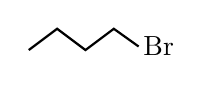
\begin{tikzpicture}[scale=0.45, baseline=-2pt]
  \draw[thick] (0,0) -- (0.8,0.6) -- (1.6,0) -- (2.4,0.6) -- (3.1,0.1) node[right=-2pt] {\ce{Br}};
\end{tikzpicture}
\end{center}
\choice
{\True $1$-bromobutane}
{$1$-bromopentane}
{$4$-bromobutane}
{$2$-bromobutane}
\loigiai{}
\end{ex}

\begin{ex}
\immini{
Catechin là một chất chống oxi hoá mạnh, ức chế hoạt động của các gốc tự do nên có khả năng phòng chống bệnh ung thư, nhồi máu cơ tim. Trong lá chè tươi, catechin chiếm khoảng $25 - 35\%$ tổng trọng lượng khô. Ngoài ra, catechin còn có trong táo, lê, nho,\dots\ Công thức cấu tạo của catechin cho như hình bên:

Phát biểu nào sau đây là \textbf{không} đúng?
}{
\setchemfig{atom sep=1.4em, bond offset=1pt}
\chemfig{*6(=(-[6]OH)-(*6(--(<[:-30]OH)-(<:[:30]*6(=-(-[:-30]OH)=(-[:30]OH)-=-))-O-))=-=(-[:150]HO)-)}
}
\choice
{\True Phân tử catechin có $5$ nhóm \ce{-OH} phenol}
{Catechin thuộc loại hợp chất thơm}
{Catechin phản ứng được với dung dịch \ce{NaOH}}
{Công thức phân tử của catechin là \ce{C15H14O6}}
\loigiai{}
\end{ex}

\begin{ex}
Trong các chất sau đây: \ce{CH3CH2OH}, \ce{CH3CHO}, \ce{CH3COOH}, \ce{CH3CH2CH2CH3}. Chất nào có nhiệt độ sôi cao nhất?
\choice
{\ce{CH3CHO}}
{\ce{CH3CH2OH}}
{\True \ce{CH3COOH}}
{\ce{CH3CH2CH2CH3}}
\loigiai{}
\end{ex}

\begin{ex}
Để phân biệt styrene và phenylacetylene có thể dùng chất nào sau đây?
\choice
{Khí oxygen dư}
{Nước bromine}
{Dung dịch \ce{KMnO4}}
{\True Dung dịch \ce{AgNO3} trong \ce{NH3}}
\loigiai{}
\end{ex}

\begin{ex}
Alkyne là những hydrocarbon mạch hở, chỉ chứa các liên kết đơn và một liên kết ba \ce{C#C} trong phân tử, có công thức chung là
\choice
{\True \ce{C_nH_{2n-2}} ($n \ge 2$)}
{\ce{C_nH_{2n+2}} ($n \ge 1$)}
{\ce{C_nH_{2n}} ($n \ge 2$)}
{\ce{C_nH_{2n-6}} ($n \ge 6$)}
\loigiai{}
\end{ex}

\begin{ex}
Geraniol có trong tinh dầu hoa hồng (công thức cấu tạo thu gọn như hình bên dưới) được sử dụng phổ biến trong công nghiệp hương liệu, thực phẩm,\dots\ vì có mùi thơm đặc trưng.
\begin{center}
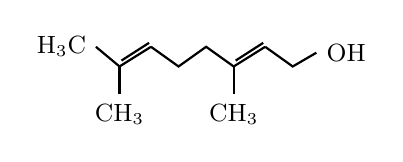
\begin{tikzpicture}[scale=0.5, font=\small, baseline=0]
  \node[left] at (-0.2,0.6) {\ce{H3C}};
  \draw[thick] (-0.2,0.6) -- (0.4,0.1);
  \draw[thick] (0.4,0.1) -- (0.4,-0.6) node[below] {\ce{CH3}};
  \draw[thick] (0.4,0.1) -- (1.2,0.6);
  \draw[thick] (0.45,0.25) -- (1.15,0.7);
  \draw[thick] (1.2,0.6) -- (1.9,0.1) -- (2.6,0.6) -- (3.3,0.1);
  \draw[thick] (3.3,0.1) -- (3.3,-0.6) node[below] {\ce{CH3}};
  \draw[thick] (3.3,0.1) -- (4.1,0.6);
  \draw[thick] (3.35,0.25) -- (4.05,0.7);
  \draw[thick] (4.1,0.6) -- (4.8,0.1) -- (5.4,0.45) node[right] {\ce{OH}};
\end{tikzpicture}
\end{center}
Geraniol thuộc loại hợp chất hữu cơ nào sau đây?
\choice
{Hydrocarbon}
{Carboxylic acid}
{\True Alcohol}
{Aldehyde}
\loigiai{}
\end{ex}

\begin{ex}
Dẫn xuất halogen nào sau đây khi tác dụng với dung dịch \ce{NaOH} đun nóng không tạo thành alcohol?
\choice
{\True \ce{C6H5Cl}}
{\ce{CH3CH(Br)CH3}}
{\ce{C6H5CH2Br}}
{\ce{C2H5Cl}}
\loigiai{}
\end{ex}

\begin{flushleft}
	{\color{blue!50!green}\fbox{\fontfamily{qag}\bfseries\selectfont PHẦN 2. Câu trắc nghiệm đúng sai}}
\end{flushleft}
\setcounter{ex}{0}
\setcounter{bt}{0}

\textit{PHẦN II. [2,0 điểm]. Thí sinh trả lời từ câu 1 đến câu 2. Trong mỗi ý a), b), c), d) ở mỗi câu, thí sinh chọn đúng (Đ) hoặc sai (S).}

\begin{ex}
Nhắc đến ethanol nhiều người thường nghĩ ngay đến đồ uống có cồn, tuy nhiên đây cũng là thành phần quan trọng được sử dụng trong y tế, là dung môi phổ biến cho nhiều ngành công nghiệp\dots
\choiceTF
{\True Ethanol còn gọi là ethyl alcohol}
{Ethanol là chất lỏng, dễ bay hơi, không mùi}
{\True Ethanol được tạo thành từ phản ứng thuỷ phân bromoethane bằng dung dịch \ce{NaOH} có đun nóng}
{\True Cho $4{,}6\text{ gam}$ ethanol tác dụng với \ce{Na} dư, thể tích khí \ce{H2} thu được (đkc) là $1{,}2395\text{ L}$}
\loigiai{}
\end{ex}

\begin{ex}
Hợp chất carbonyl đơn giản nhất là aldehyde và ketone đơn chức. Chúng có nhiều ứng dụng trong ngành công nghiệp hoá chất cũng như trong thiên nhiên.
\choiceTF
{Cho $0{,}44\text{ gam}$ ethanal vào dung dịch \ce{AgNO3} trong \ce{NH3} dư, đến khi phản ứng hoàn toàn thì thu được $10{,}8\text{ gam}$ \ce{Ag}}
{\True Trong tinh dầu thảo mộc có chứa những aldehyde, dùng dung dịch \ce{AgNO3} trong \ce{NH3} để nhận biết thành phần aldehyde trong tinh dầu}
{Tên thay thế của \ce{(CH3)2CHCH2CHO} là $2$-methylbutanal}
{Ethanal và propanone không thuộc loại hợp chất carbonyl}
\loigiai{}
\end{ex}

\begin{flushleft}
	{\color{blue!50!green}\fbox{\fontfamily{qag}\bfseries\selectfont PHẦN 3. Câu trắc nghiệm trả lời ngắn}}
\end{flushleft}
\setcounter{ex}{0}
\setcounter{bt}{0}

\textit{PHẦN III. [2,0 điểm]. Câu trắc nghiệm yêu cầu trả lời ngắn. Thí sinh trả lời từ câu 1 đến câu 4.}

\begin{ex}
Ethene và acetylene là những hydrocarbon không no đơn giản nhất và có nhiều ứng dụng quan trọng. Một ứng dụng quan trọng của acetylene là làm nhiên liệu trong đèn xì oxygen - acetylene. Khi đèn hoạt động, hai khí này được trộn vào nhau để thực hiện phản ứng đốt cháy theo sơ đồ \ce{C2H2 + O2 ->[t^o] 2CO2 + H2O}. Đốt cháy hoàn toàn $V\text{ lít}$ (đkc) khí acetylene thu được $7{,}2\text{ gam}$ \ce{H2O}. Nếu cho tất cả sản phẩm cháy hấp thụ hết vào bình đựng nước vôi trong dư thì khối lượng bình tăng $m\text{ gam}$. Tính giá trị của $m$?
\par\shortans[oly]{42{,}4}
\loigiai{}
\end{ex}

\begin{ex}
Phenol được dùng để sản xuất phẩm nhuộm, nhựa phenol-formaldehyde, thuốc nổ ($2{,}4{,}6$-trinitrophenol), chất diệt cỏ 2,4-D, chất diệt nấm mốc (các đồng phân của nitrophenol),\dots\ Do có tính diệt khuẩn nên phenol được dùng làm chất khử trùng, tẩy uế. Thuốc xịt chloraseptic chứa $1{,}4\%$ phenol được dùng làm thuốc chữa đau họng. Cho các phát biểu sau:
\begin{enumerate}[a)]
	\item Phenol tan vô hạn trong nước lạnh ở điều kiện thường.
	\item Nhiệt độ nóng chảy của phenol cao hơn ethanol.
	\item Phenol có khả năng tác dụng với dung dịch bromine tạo kết tủa trắng.
	\item Phenol dùng để sản xuất phẩm nhuộm, chất diệt nấm mốc, thuốc nổ TNT.
\end{enumerate}
Có bao nhiêu phát biểu đúng?
\par\shortans[oly]{2}
\loigiai{}
\end{ex}

\begin{ex}
Ngày nay, nhu cầu về đồ gỗ nội thất ngày càng nhiều song nguồn gỗ tự nhiên không còn dồi dào nên việc chuyển sang sử dụng gỗ công nghiệp đang là xu hướng của nhiều nước trên thế giới. Việc sử dụng gỗ công nghiệp góp phần bảo vệ rừng, bảo vệ môi trường. Quy trình sản xuất gỗ công nghiệp là nghiền các cây gỗ trồng ngắn ngày như keo, bạch đàn, cao su,\dots, sau đó sử dụng keo để kết dính và ép để tạo độ dày ván gỗ. Keo được sử dụng trong gỗ công nghiệp thường chứa dư lượng formaldehyde, là một hoá chất độc hại đối với sức khoẻ con người. Tại các nước phát triển như ở châu Âu và Mỹ, dư lượng formaldehyde được kiểm soát rất nghiêm ngặt. Châu Âu quy định tiêu chuẩn dư lượng formaldehyde trong gỗ công nghiệp là $120\ \mu\mathrm{g}\cdot\mathrm{m}^{-3}$. Cơ quan kiểm định lấy $300\text{ gam}$ gỗ trong một lô gỗ của một doanh nghiệp Việt Nam xuất khẩu sang châu Âu và kiểm tra bằng phương pháp sắc kí thấy chứa $0{,}03\ \mu\mathrm{g}$ formaldehyde. Biết khối lượng riêng của loại gỗ này là $800\ \mathrm{kg}\cdot\mathrm{m}^{-3}$. Hàm lượng formaldehyde có trong $800\text{ kg}$ (hay $1\ \mathrm{m}^3$) gỗ là bao nhiêu $\mu\mathrm{g}$?
\par\shortans[oly]{80}
\loigiai{}
\end{ex}

\begin{ex}
Cho các chất sau: \ce{H-CHO}; \ce{H-COOH}; \ce{CH3-COOH}; \ce{C2H5-OH}; \ce{CH2=CH-COOH}; \ce{C6H5-COOH}; \ce{HOOC-COOH}; \ce{C6H6}; \ce{HOOC-CH2-COOH}; \ce{C2H5COOH}.\\
Có bao nhiêu hợp chất carboxylic acid trong các chất trên?
\par\shortans[oly]{7}
\loigiai{}
\end{ex}

\smallskip
\noindent
\textbf{B. PHẦN TỰ LUẬN: [3,0 điểm]}

\begin{flushleft}
	{\color{blue!50!green}\fbox{ \fontfamily{qag}\bfseries\selectfont Tự Luận:}}
\end{flushleft}
\setcounter{ex}{0}
\setcounter{bt}{0}

\begin{ex}
\textbf{[1,0 điểm]} Các nhà hoá học đã tìm ra một số dẫn xuất halogen không chứa chlorine như: \ce{CBr2F2}, \ce{CF3-CHF2}, \ce{CH2=CF-CF3}, \ce{CF3CH2CF2CH3},\dots\ đang được sử dụng trong công nghiệp nhiệt lạnh, vì sự phân huỷ các hợp chất này nhanh chóng sau khi phát tán vào không khí nên ảnh hưởng rất ít đến tầng ozone hay sự ấm lên toàn cầu thấp. Gọi tên theo danh pháp thay thế các hợp chất đó.
\loigiai{}
\end{ex}

\begin{ex}
\textbf{[1,0 điểm]} Trong công nghiệp chế biến đường từ mía sẽ tạo ra sản phẩm phụ, gọi là rỉ đường hay rỉ mật, sử dụng rỉ đường để lên men tạo ra ethanol trong điều kiện thích hợp, hiệu suất cả quá trình là $80\%$. Tính khối lượng ethanol thu được từ $1{,}5\text{ tấn}$ rỉ đường mía theo 2 phương trình:
$$\ce{C12H22O11 + H2O -> C6H12O6 + C6H12O6}$$
$$\ce{C6H12O6 -> 2C2H5OH + 2CO2}$$
\loigiai{}
\end{ex}

\begin{ex}
\textbf{[1,0 điểm]} Thị trường tiêu thụ phenol trên toàn thế giới khoảng $11{,}67\text{ triệu tấn}$ trong năm 2022. Phenol được sử dụng để sản xuất nhiều loại hoá chất như bisphenol A, nhựa phenol-formaldehyde, picric acid và các chất khác. Khoảng $90\%$ lượng phenol được sản xuất từ cumene. Khối lượng cumene cần dùng để sản xuất phenol cho năm 2022 là bao nhiêu?
\loigiai{}
\end{ex}

\begin{center}
\textbf{---------- HẾT ----------}
\end{center}

\smallskip
\noindent
\begin{tabular}{ll}
- & Thí sinh không được sử dụng tài liệu.\\
- & Cán bộ coi kiểm tra không giải thích gì thêm.
\end{tabular}

\end{document}
